\section{2点関数}
\subsection{シュウィンガー・ダイソン方程式}
\begin{figure}[ht]
  \centering
  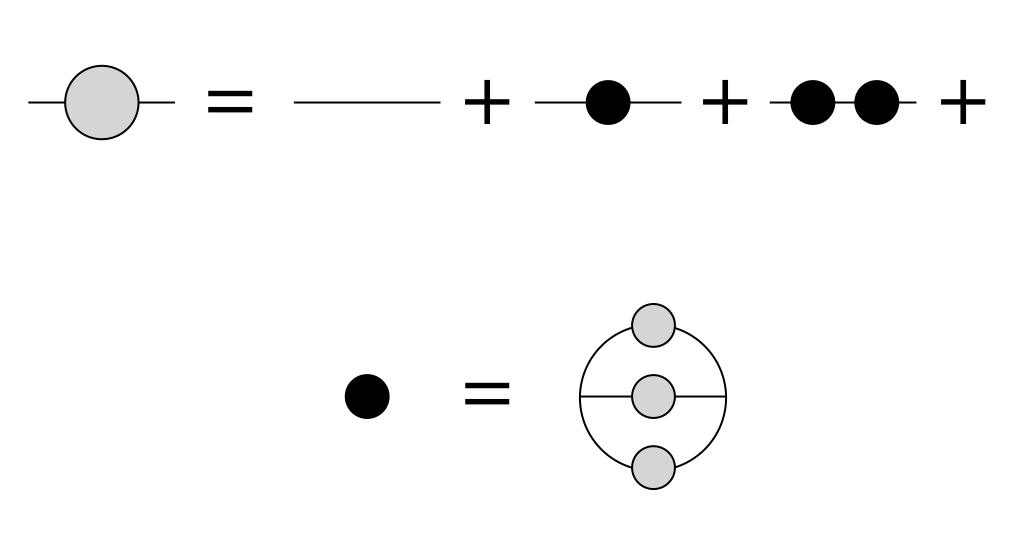
\includegraphics[width=14cm]{figures/melonDiagram}
  \caption{ラージN極限において2点関数に寄与する最初の補正ダイアグラム.
  特に$q=4$の場合について描画している. 灰色の丸と黒い丸はそれぞれ完全な2点関数および
  1粒子相互作用を表している.}
  \label{fig:melonDiagram}
\end{figure}

SYK模型の作用は
\begin{align}
  I = \int dt\ \left(\frac{1}{2}\sum_{i = 1}^{N} \psi_i \deriv \psi_i
		- \frac{1}{4!} \sum_{i,j,k,l = 1}^{N} J_{ijkl} \psi_i\psi_j\psi_k\psi_l
    \right)
\end{align}
である。
これを$J_{ijkl}$について期待値を取り、その後フェルミオンを積分するために
2つのbi-local場$G(t_1, t_2)$, $\Sigma(t_1, t_2)$を導入すると
\begin{align}
  \frac{I_{\mathrm eff}}{N} =
		- \frac{1}{2}\log\det\left(\deriv - \Sigma\right)
		+ \frac{1}{2}\int dt_1dt_2\ \left(\Sigma G - \frac{J^2}{4}G^4\right)
  \label{eq:effectiveAction}
\end{align}
を得る\footnote{詳しい計算は\ref{app:effective_action}を参照すること.}。
\eqref{eq:effectiveAction}式の停留点が次式のシュウィンガー・ダイソン方程式を与える:
\begin{align}
  G(\omega)^{-1} = -i\omega - \Sigma(\omega),
  \hspace{30pt}
  \Sigma(t) = J^2G(t)^3
  \label{eq:SDeq}
\end{align}

なお、SYK模型では4つのフェルミオンが相互作用するとしているが、その数を$q$として一般化しても
有効作用やシュウィンガー・ダイソン方程式は計算する事ができ、それぞれ
\begin{align}
  \frac{I_{\mathrm eff}}{N} =
		- \frac{1}{2}\log\det\left(\deriv - \Sigma\right)
		+ \frac{1}{2}\int dt_1dt_2\ \left(\Sigma G - \frac{J^2}{q}G^q\right)
  \label{eq:effectiveActionWithGeneral_q}
\end{align}
\begin{align}
  G(\omega)^{-1} = -i\omega - \Sigma(\omega),
  \hspace{30pt}
  \Sigma(t) = J^2G(t)^{q-1}
  \label{eq:SDeqWithGeneral_q}
\end{align}
である。さらに複数の$q$について相互作用項を足し合わせたような一般化したSYK模型も
調べられており、\cite{gross}にて詳しく論じられている。

ラージ$N$極限を施したSYK模型において、リーディングオーダーで2点関数に寄与する
ファインマンダイアグラムは「メロンダイアグラム」と呼ばれている
\footnote{このメロンはwatermelonのmelonであってメロンではないらしい.
どの辺がスイカなのかはよく分からない.}。
\eqref{eq:SDeqWithGeneral_q}式の一般の$\omega$における解析的な計算は現在のところ
知られていないが、数値的には可能であり、図\ref{fig:melonDiagram}のダイアグラムのように
再帰的に計算を走らせる事で2点関数のグラフをプロットできる。

\begin{figure}[ht]
	\begin{tabular}{cc}
		\begin{minipage}[t]{0.45\hsize}
			\centering
			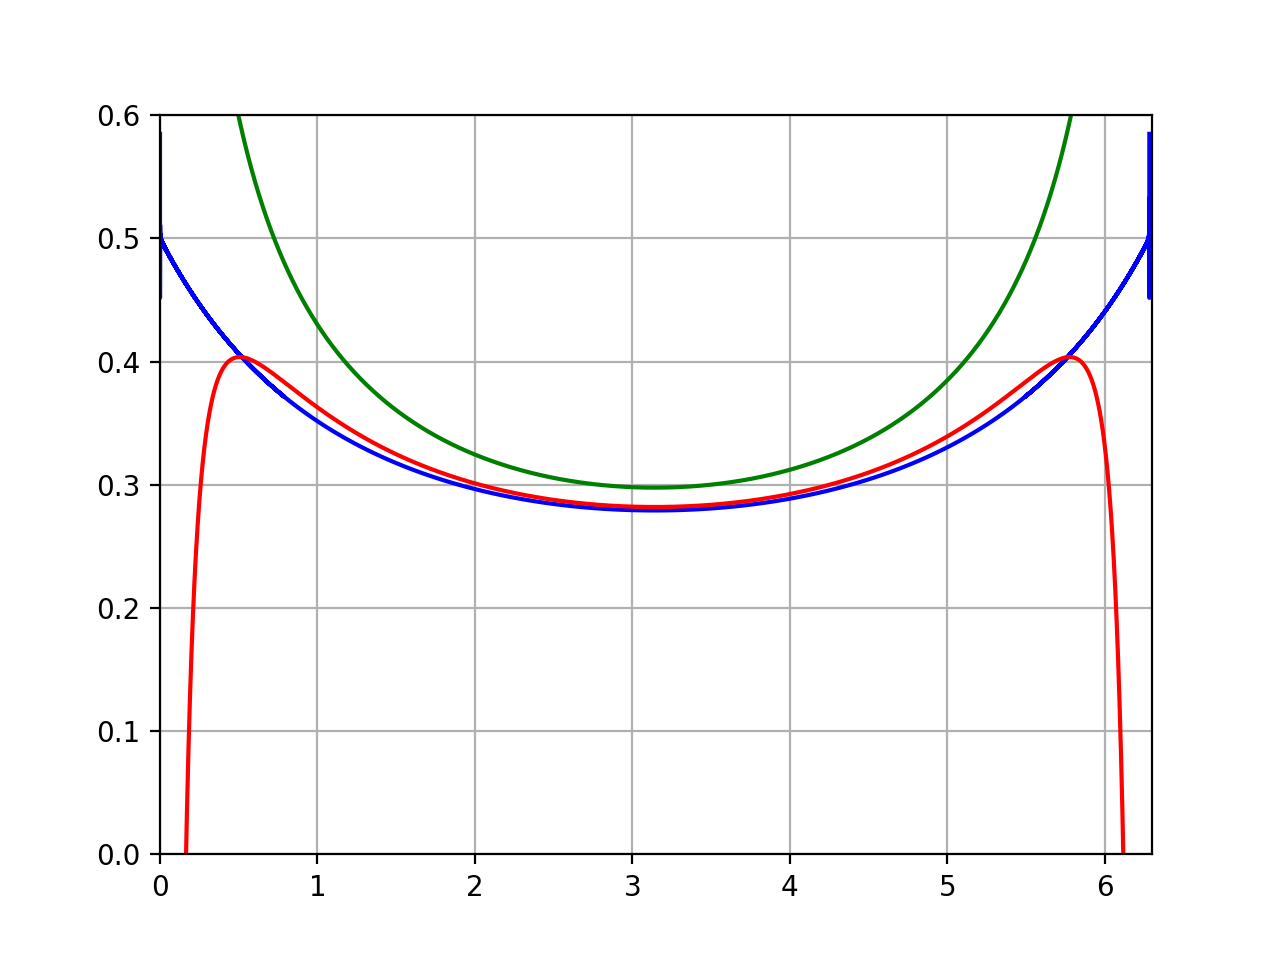
\includegraphics[width=8cm]{figures/J10}
			\caption{$J = 10$としてプロットした2点関数. 横軸は時間である. 
			青色の線が一般の$\omega$, 緑色の線が$\omega = 0$, 
			赤色の線が低エネルギー極限に$J^{-1}$補正を加えたものである.}
			\label{fig:J10}
		\end{minipage}
		\begin{minipage}[t]{0.45\hsize}
			\centering
			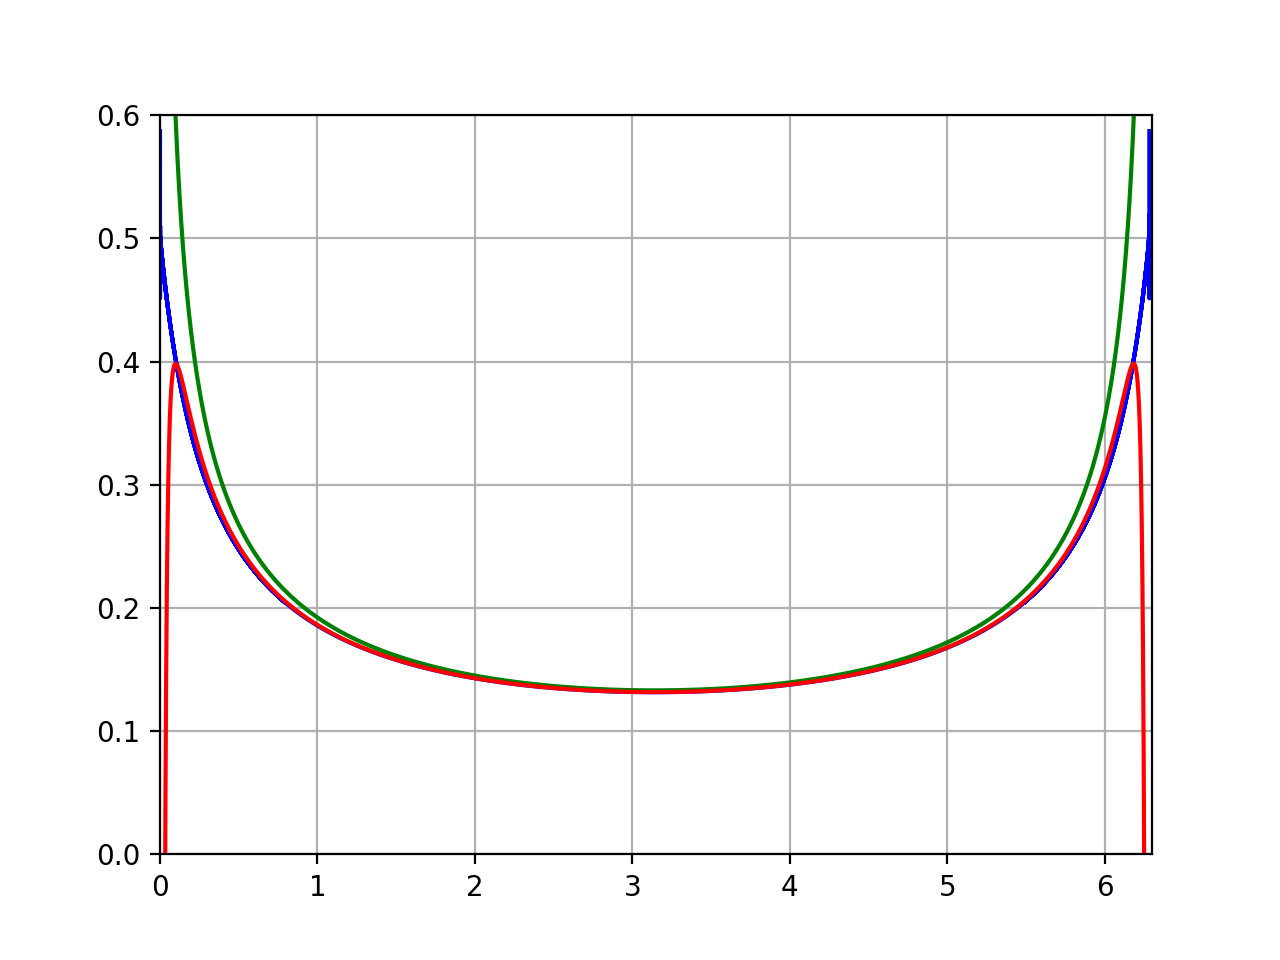
\includegraphics[width=8cm]{figures/J50}
			\caption{$J = 50$としてプロットした2点関数. 横軸は時間である. 各色の意味は左図と同様. 
				低エネルギー極限はラージ$J$極限でもあるので, 左図と比べて各線は互いに近づく.}
			\label{fig:J50}
		\end{minipage}
	\end{tabular}
\end{figure}

\subsection{共形不変性}
シュウィンガー・ダイソン方程式\eqref{eq:SDeqWithGeneral_q}は$\omega = 0$という
低エネルギー極限においては解析的な解が知られている。
この時\eqref{eq:SDeqWithGeneral_q}式の一つ目の式は
\begin{align}
	\Sigma(\omega)G(\omega) = -1
\end{align}
となり、この両辺にフーリエ変換を施す事でシュウィンガー・ダイソン方程式は
\begin{align}
	\int dt\ G(t_1, t)\Sigma(t, t_2) = -\delta(t_1 - t_2),
	\hspace{30pt}
	\Sigma(t_1, t_2) = J^2 (G(t_1, t_2))^{q-1}
	\label{eq:conformalSD}
\end{align}
と書き改める事ができる.
これらの2つの式は次のようなパラメータ付け替え不変性を持つ:
\begin{align}
	G(t_1, t_2) \to (f(t_1)f(t_2))^{\Delta}G(f(t_1),f(t_2)),
	\hspace{20pt}
	\Sigma(t_1, t_2) \to (f(t_1)f(t_2))^{1 - \Delta}\Sigma(f(t_1),f(t_2)).
\end{align}
ここで$\Delta = 1 / q$である。
我々は解として次のような形を仮定する:
\begin{align}
	G_c(t) = \frac{b}{|t|^{2\Delta}}\mathrm{sgn}(t),
	\hspace{20pt}
	\mathrm{or}
	\hspace{20pt}
	G_c(t) = b\left[\frac{\pi}{\beta\sin(\pi t / \beta)}\right]^{2\Delta}\mathrm{sgn}(t)
	\label{eq:conformal_ansatz}
\end{align}
2番目の式は有限温度の場合の解であり、パラメータ$t$を$f(t) = \tan(\pi t / \beta)$と変換して得る。
図\ref{fig:J10}および図\ref{fig:J50}において$G_c$を緑色の線でプロットしたところ、一般の$\omega$からは少しずれた。
係数$b$は
\begin{align}
	J^2 b^q \pi = \left(\frac{1}{2} - \Delta \right)\tan(\pi \Delta)
\end{align}
から決める事ができる\footnote{詳しくは\ref{app:b}を参照.}。

\subsection{ラージ$q$極限}

\subsubsection{リーディングオーダー}

\subsubsection{サブリーディングオーダー}





\pagebreak
